\clearpage
\section{Noise Characterization}\label{section:noise_characterization}

The most important factor of the system is its noise behavior. It directly poses limits on the operating conditions within which the device is accurate enough and thus defines its usability and reliability in the most difficult and life-threatening situations. As no system is perfect, this chapter focuses on defining an acceptable noise level based on the specification, system design and the noise performance of the algorithm used.

\subsection{Noise Requirements}

The ISO 80601-2-61 standard defines a baseline of performance requirements for \spo monitoring that GE devices should meet \cite{ISO80601-2-612011}, but more importantly, competitors' devices claim to achieve even better performance. Masimo and Covidien (Nellcor) both report an RMS overall error of 2 percentage points in the \spo reading with IR modulation as low as 0.03\% \cite{Tram_spec}, which means that it's good business for GE to top that figure. Therefore the goal is to stay below 2 percentage points of error down to IR modulation of 0.02\%. This imposes a strict requirement for the system's noise behavior since a signal that weak can easily be lost in the noise floor, depending on the algorithm used.

The simplest algorithm to use for calculating R (equation \ref{eq:ratio_of_ratios}) is the peak-to-peak algorithm: the signal is analyzed and the values for $I_{AC}$ and $I_{DC}$ are found by recording the maximum, minimum and mean values of the signals. In this case the peak-to-peak noise present in the full frequency band of interest affects the measurement directly, thus skewing the \spo result. As the pleth signal is usually in the range of 0.5-20 Hz, the dominating noise type can be either white or 1/f.

The formulation of the noise requirement for the system can be started with deriving the equation (\ref{eq:ratio_of_ratios}) and assuming that the noises in the two channels sum up in a root-mean-square manner:

\begin{equation}
\begin{array}{l}
	\left\{
	  \begin{array}{l c c l}
	      & \frac{dR}{dI_{AC,R}} &=& \frac{I_{DC,IR}}{I_{AC,IR} \cdot I_{DC_R}} \\
	      & \frac{dR}{dI_{AC,IR}} &=& - \frac{I_{AC,R} \cdot I_{DC,IR}}{I_{AC,IR}^2 \cdot I_{DC,R}} \\
	      & \Delta R &=& \sqrt{(I_{n,R} \cdot \frac{dR}{dI_{AC_R}})^2 + (I_{n,IR} \cdot \frac{dR}{dI_{AC,IR}})^2}
	  \end{array} \right. \\
	
	\rightarrow \Delta R = \sqrt{I_{n,R}^2 + (I_{n,IR} \cdot \frac{I_{AC,R}}{I_{AC,IR}})^2} \cdot \frac{I_{DC,IR}}{I_{AC,IR} \cdot {I_{DC,R}}}
\end{array}
\label{eq:dR}
\end{equation}

By defining the signal modulation ratios and assuming that the signals can be controlled so that they are at the same DC level it can be concluded that

\begin{equation}
  \begin{array}{l}
	  \left\{
	  \begin{array}{c c c c l}
	  	 m &=& \frac{I_{AC}}{I_{DC}} & & \\
	  	 m_{R} &=& R \cdot m_{IR} & & \\
	  	 I_{DC,R} &=& I_{DC,IR} &=& I_{DC}
	  \end{array} \right. \\
	  \\
		\begin{array}{r c l}
			\Delta R &=& \sqrt{I_{n,R}^2 + (I_{n,IR} \cdot R)^2} \cdot \frac{1}{I_{AC,IR}} \\
			& & \\
			\Delta R &=& \frac{\sqrt{I_{n,R}^2 + (I_{n,IR} \cdot R)^2}}{I_{DC} \cdot m_{IR}}
		\end{array}
	\end{array}
	\label{eq:DeltaR}
\end{equation}

Equation \ref{eq:DeltaR} states that the error in R imposed by noise is directly proportional to the noise level and inversely proportional to the signal level and modulation ratio. The specification determines the minimum modulation ratio but the optimal signal level is defined by the system's dynamic behavior; usually the signal is kept in the middle of the ADC's dynamic range, leaving room for detecting motion and other artifacts, but the better the system the closer the signal can be kept to the high limit of the range.

For the sake of simplification it's assumed that the noise magnitude is the same for each channel, which is also true on average. Therefore the equation reduces itself to a form that will be used in further calculations:

\begin{equation}
	\Delta R = \sqrt{1 + R^2} \cdot \frac{I_{n,pp}}{I_{DC} \cdot m_{IR}} .
	\label{eq:DeltaRSymmetric}
\end{equation}

As explained in section \ref{section:pulse_oximetry}, R maps to an \spo reading with a non-linear relation. Calibration data is used for this mapping but usually the relationship is the form of an equation of 2nd degree, and said equation can also be used to find the relation between the error in R and the error in \spo:

%\begin{equation}
%\begin{array}{c c l}
%	S_pO_2(R) &=& aR^2 + bR + c \\
%	\Delta S_pO_2(R) &=& S_pO_2(R) - S_pO_2(R + \Delta R) \\
%	                 &=& aR^2 + bR + c - a(R+\Delta R)^2 - bR - b \Delta R - c \\
%	                 &=& a(R^2 - R^2 - 2 R \Delta R - (\Delta R)^2) - b \Delta R \\
%	                 &=& -((2aR + b) \cdot \Delta R + a (\Delta R)^2)
%\end{array}
%\label{eq:DeltaSpO2}
%\end{equation}

\begin{equation}
  \begin{array}{ccl}
    \spo(R) &=& aR^2 + bR + c \\
    R(\spo) &=& \frac{-b - \sqrt{b^2 - 4a(c-\spo)}}{2a} \\
    & & \\
    \Delta R(\spo, \Delta\spo) &=& R(\spo + \Delta\spo) - R(\spo) \\
    & & \\
    \Delta R(\spo, \Delta\spo) &=& \frac{\sqrt{b^2 - 4a(c-\spo)} - \sqrt{b^2 - 4a(c - \spo - \Delta\spo)}}{2a}
  \end{array}
  \label{eq:DeltaRspo}
\end{equation}    

By combining equations (\ref{eq:DeltaRSymmetric}) and (\ref{eq:DeltaRspo}), fixing \spo tolerance and solving the equation in respect to $I_n$ a relationship is established between the performance specification and allowed noise level:

%\begin{equation}
%\begin{array}{c c l}
%  \Delta S_pO_2 &=& - I_{noise} \cdot \frac{(1+R) \cdot (2aR + b)}{I_{DC} \cdot m_{IR}} - I_{noise}^2 \cdot \frac{a \cdot (1+R)^2}{I_{DC}^2 \cdot m_{IR}^2} \\
%  0 &=& I_{noise}^2 \cdot \frac{a \cdot (1+R)^2}{I_{DC}^2 \cdot m_{IR}^2} + I_{noise} \cdot \frac{(1+R) \cdot (2aR + b)}{I_{DC} \cdot m_{IR}} + \Delta S_pO_2 \\
%  & & \\
%  I_{noise}(R) &=& - \frac{ \frac{(2aR + b)(1+R)}{I_{DC} m_{IR}} \mp \sqrt{\frac{(2aR+b)^2(1+R)^2}{I_{DC}^2 m_{IR}^2} - 4a \frac{(1+R)^2}{I_{DC}^2 m_{IR}^2} \cdot \Delta S_pO_2} }{ %2a \frac{(1+R)^2}{I_{DC}^2 m_{IR}^2} }\\
%  & & \\
%  I_{noise}(R) &=& \frac{-2aR - b \mp \sqrt{(2aR + b)^2 - 4a \cdot \Delta S_pO_2}}{\frac{2a(1+R)}{I_{DC} m_{IR}}} \\
%  & & \\
%  I_{noise}(R) &=& \frac{(-2aR - b \mp \sqrt{(2aR + b)^2 - 4a \cdot \Delta S_pO_2}) \cdot I_{DC} \cdot m_{IR}}{2a(1+R)}
%\end{array}
%\label{eq:maximum_noise}
%\end{equation}

\begin{equation}
  \begin{array}{ccl}
    I_n(\spo) &=& I_{DC} \cdot m_{IR} \cdot \frac{\Delta R(\spo, \Delta\spo)}{\sqrt{1 + R^2(\spo)}} \\
    & & \\
    I_n(\spo) &=& I_{DC} \cdot m_{IR} \cdot \frac{\sqrt{b^2 - 4a(c-\spo)} - \sqrt{b^2 - 4a(c - \spo - \Delta\spo)}}
    {\sqrt{4a^2 - 4a(c-\spo) + 2b^2 + 2b \sqrt{b^2 - 4a(c-\spo)}}}
  \end{array}
  \label{eq:maximum_noise}
\end{equation}

%Finally, using the relationship between \spo and R, the equation reaches the following form:
%\begin{equation}
% \begin{array}{c c l}
%  R(\spo) &=& \frac{-b - \sqrt{b^2 - 4a(c - \spo)}}{2a} \\
%  \\
%  I_{noise}(\spo) &=& \frac{(\sqrt{b^2 - 4a(c - \spo)} \mp \sqrt{b^2 - 4a(c - \spo + \Delta\spo)}) \cdot I_{DC} \cdot m_{IR}}{2a - b - \sqrt{b^2-4a(c - \spo)}}
% \end{array}
% \label{eq:max_noise_vs_spo2}
%\end{equation}

The overall noise tolerance of the system is the minimum of the function above. The function solved with values defined in table \ref{tbl:specification_constants} is plotted in figure \ref{fig:noise_requirement_vs_spo2}. It's to be noted, though, that the tolerance figure includes all calibration errors, motion and respiratory artifacts and other sources of error -- therefore the signal path itself should introduce even less noise for the system to fulfill the requirements in normal operating conditions. Based on data gathered from previous GE oximeter designs it's estimated that most, but not all, of the total error is due to additive noise in the signal path and the rest is from other sources; if the allowed 1-$\sigma$ tolerance in the \spo value due to signal path noise is defined to be 1 \%-point, the required signal-to-noise ratio calculated using the same method is approximately 127 dB. Assuming white spectrum, the peak-to-peak noise is converted to RMS noise by dividing by 6.6 for the calculation of SNR.

\begin{table}[htcb]
  \begin{center}
  \caption{Example calibration values and performance specification constants}
	\begin{tabular}{|c|c|c|}
		\hline
		\textbf{Item} & \textbf{Symbol} & \textbf{Value} \\
		\hline
		Calibration coefficient & a     & -6.68  \\
		\hline
		Calibration coefficient & b     & -19.9  \\
		\hline
		Calibration coefficient & c     & 112    \\
		\hline
		IR Modulation Ratio & $m_{IR}$  & 0.0002 \\
		\hline
		Signal Level  & $I_{DC}$        & 5 $\mu A$ \\
		\hline
		Output tolerance & $\Delta \spo$ & $\pm1$ \%-point\\
		\hline
		Output range     & \spo & 70--100 \% \\
		%\hline
		%Range of R (calculated with a, b and c) & R & [0.5, 1.43] \\
		\hline
		Pleth power distribution coefficient & $\alpha$ & 0.3 \\
		\hline
		Noise power distribution coefficient & $\beta$  & $\frac{1}{64}$ \\
		\hline
	\end{tabular}
	\label{tbl:specification_constants}
	\end{center}
\end{table}

\begin{figure}[htcb]
  \begin{center}
  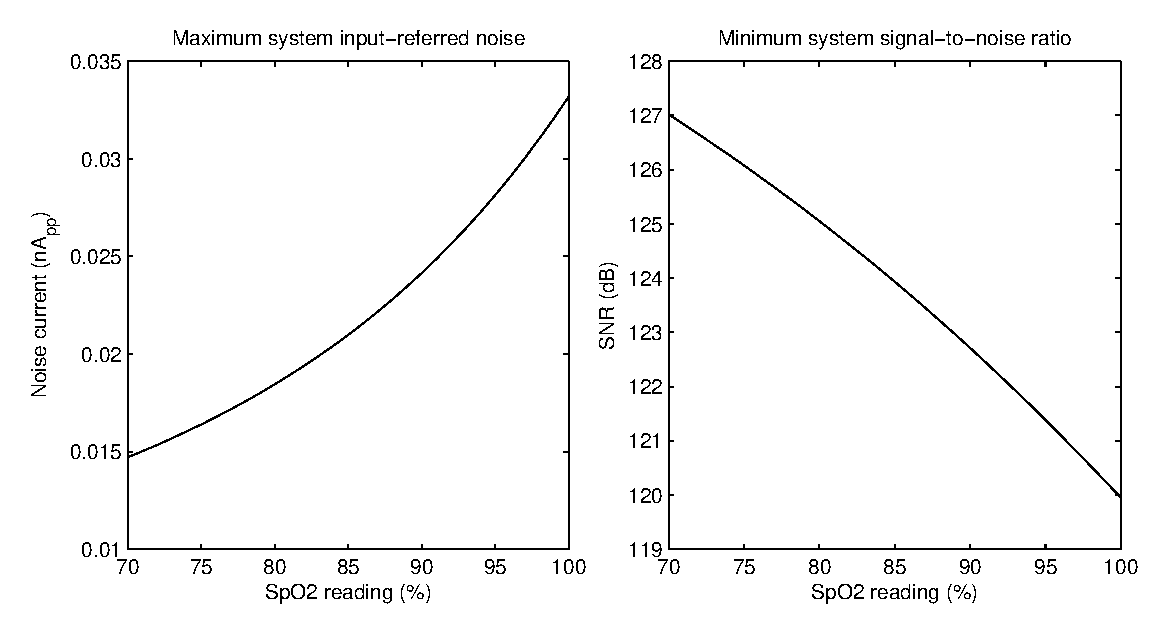
\includegraphics[scale=0.8]{kuvat/noise_requirement_vs_spo2.eps}
  \caption{The system's maximum noise level as a function of \spo reading according to equation \ref{eq:maximum_noise} and table \ref{tbl:specification_constants}.}
  \label{fig:noise_requirement_vs_spo2}
  \end{center}
\end{figure}

\subsection{\spo Algorithm and Noise}

As mentioned previously, the peak-to-peak algorithm in time domain is the simplest one to implement but also the most prone to be disturbed by noise. Fortunately there are alternatives, the more advanced taking advantage of the rhythmic nature of the plethysmographic signal and working in frequency domain.

The frequency domain approach used by GE periodically processes a 5-second window of the signal by performing a Fast Fourier Transform (FFT) on it and seeking the strongest frequency spike to act as the AC signal, similarly to \cite{Scharf1993}. The benefit of this approach is that since most of the pleth signal's energy is focused on the fundamental frequency it captures the signal properties quite well but is only affected by noise on that specific frequency. This means that most of the white or pink noise present in the system goes unnoticed -- the actual advantage gained depends on the frequency step of the FFT and the relationship between noise spectrum and cardiac frequency but effective noise can usually be reduced by a noticeable factor compared to algorithms working in time domain.

\begin{figure}[htcb]
\begin{center}
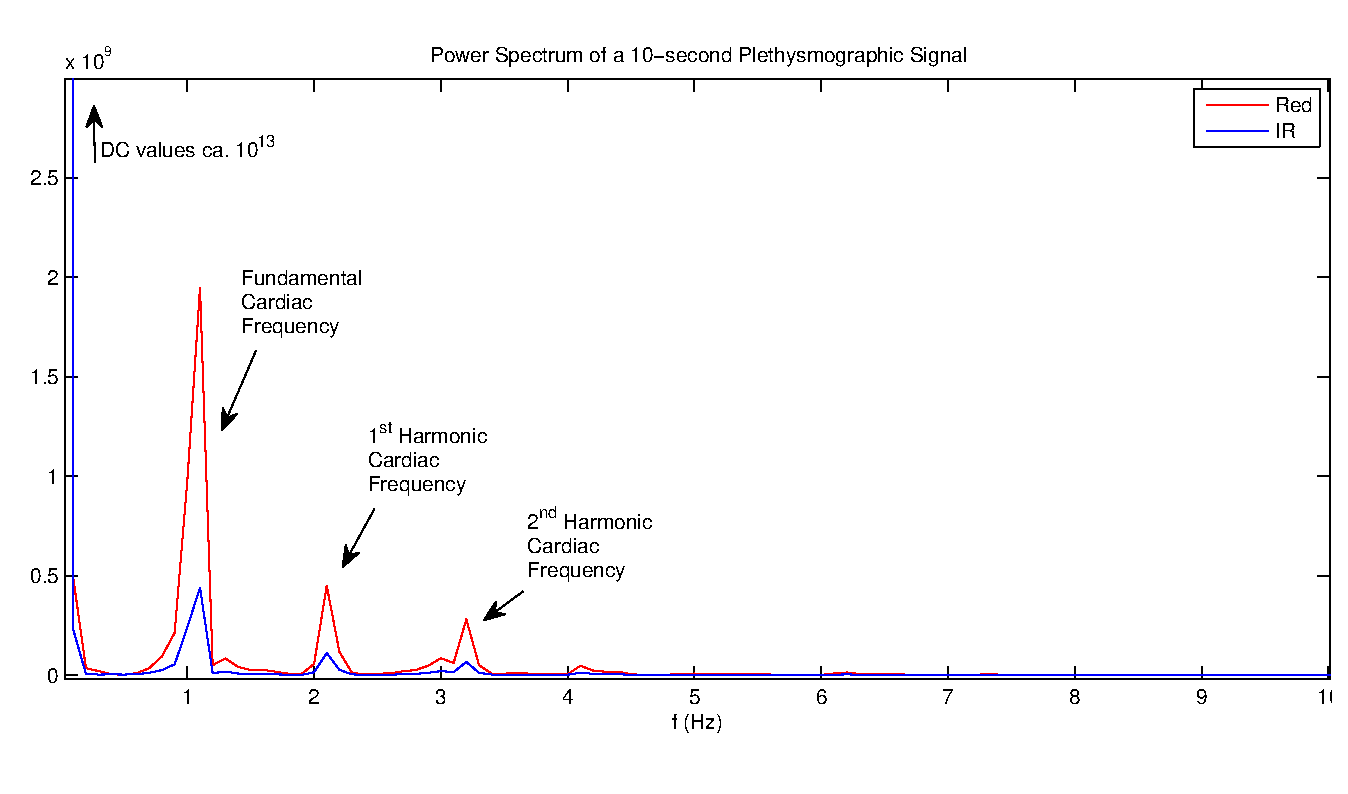
\includegraphics[scale=0.6]{kuvat/pleth_power_spectrum.eps}
\caption{The power spectrum of a typical strong plethysmographic signal showing the fundamental cardiac frequency and its harmonics.}
\label{fig:pleth_power_spectrum}
\end{center}
\end{figure}

Figure \ref{fig:pleth_power_spectrum} shows the power spectrum of a typical strong plethysmographic signal windowed to 10 seconds. It's clearly seen that the fundamental cardiac frequency and its harmonics are the dominant components and raise well above any noise levels. The powers of the fundamental frequencies in both channels can directly be divided with the zero-hertz powers and each other to calculate $R$, $\alpha$ denoting the portion of pleth signal power focused on the fundamental frequency:

\begin{equation}
\left\{
	\begin{array}{cclcl}
		R &=& \frac{m_{R}}{m_{IR}} &=& \sqrt{\frac{\frac{P_{f,R}}{P_{0,R}}}{\frac{P_{f,IR}}{P_{0,IR}}}} \\
		X_{f} &=& \left| \sum\limits_{n=0}^{N-1}{x_n e^{-i2\pi \frac{f}{f_s} \frac{n}{N}}} \right| &\approx& \frac{N}{2} \sqrt{\alpha} I_{AC} \\
		P_f &=& X_{f}^2 &\approx& \frac{N^2}{4} \alpha I_{AC}^2 \\
		P_0 &=& P_{0,R} = P_{0,IR} &=& N^2 I_{DC}^2
	\end{array}
\right .
\end{equation}
\begin{equation}
\rightarrow R = \sqrt{\frac{X^2_{f,R}}{X^2_{f,IR}}} = \frac{X_{f,R}}{X_{f,IR}}
\end{equation}

The square root is necessary to reduce the ratio of powers to a ratio of amplitudes. Alternatively, the relation between \spo and the calculated ratio could be modified accordingly. Further on, the equation can be derived like done in equation (\ref{eq:DeltaR}) to formulate the noise requirement, taking into account the noise reduction coefficient $\beta$ achieved from the FFT and assuming that the noises in the two channels will add up in RMS fashion:

\begin{equation}
\left\{
	\begin{array}{ccl}
		\Delta X_f &=& \frac{N}{2} \cdot \sqrt{\beta} \cdot I_{n} \\
	  & & \\
	  %\frac{dP_f}{dI_{AC}} &=& 2 \alpha I_{AC} \\
	  \frac{dR}{dX_{f,R}}  &=& \frac{1}{X_{f,IR}} \\
	  & & \\
	  \frac{dR}{dX_{f,IR}} &=& - \frac{X_{f,R}}{X^2_{f,IR}} = - \frac{R}{X_{f,IR}} \\
	  & & \\
	  \Delta R(\Delta X_f) &=& \sqrt{(\Delta X_{f} \cdot \frac{dR}{dX_{f,R}})^2 + (\Delta X_{f} \cdot \frac{dR}{dX_{f,IR}})^2} 
	\end{array}
\right .
\end{equation}
\begin{equation}
  \begin{array}{rcl}
    \rightarrow \Delta R &=& \Delta X_f \sqrt{\frac{1}{X_{f,IR}^2} + \frac{R^2}{X_{f,IR}^2}} \\
    &=& \frac{\Delta X_f}{X_{f,IR}} \cdot \sqrt{1 + R^2} \\
    &=& \frac{2 N \sqrt{\beta} I_n}{2 N \sqrt{\alpha} I_{AC,IR}} \cdot \sqrt{1 + R^2} \\
    \Delta R &=& \sqrt{\frac{\beta}{\alpha}} \cdot \frac{I_n}{I_{DC} \cdot m_{IR}} \cdot \sqrt{1 + R^2}
  \end{array}
\end{equation}
\begin{equation}
  \rightarrow I_n(S_pO_2) = \sqrt{\frac{\alpha}{\beta}} \cdot I_{DC} \cdot m_{IR} \cdot \frac{\Delta R(S_pO_2)}{\sqrt{1 + R(S_pO_2)^2}}
  \label{eq:max_noise_vs_DeltaR_fft}
\end{equation}

%% Vaihtoehtoinen l�hestymistapa. K�ytet��n kuitenkin tehopohjaista.
%  From these it can be concluded that 
%  \begin{equation}
%    \begin{array}{cccl}
%	    & \frac{dR}{dI_{AC,R}} &=& \frac{dR}{dP_{f,R}} \frac{dP_{f,R}}{dI_{AC,R}} = \sqrt{\frac{\alpha P_{0,IR}}{P_{f,IR} P_{0,R}}} = \sqrt{\frac{\alpha}{P_{f,R}}} \cdot R \\
%	    & & & \\
%	    \rightarrow & \frac{dR}{dI_{AC,R}} &=& \frac{R}{I_{AC,R}} = \frac{\frac{m_R}{m_{IR}}}{I_{DC} \cdot m_{R}} = \frac{1}{I_{DC} \cdot m_{IR}}
%    \end{array}
%  \end{equation}
%
%  and
%
%  \begin{equation}
%    \begin{array}{ccl}
%	    \frac{dR}{dI_{AC,IR}} &=& \frac{dR}{dP_{f,IR}} \frac{dP_{f,IR}}{dI_{AC,IR}} = - \sqrt{\alpha P_{f,IR}} \cdot \sqrt{\frac{P_{f,R} P_{0,IR}}{P_{f,IR}^3 P_{0,R}}} \\
%	    & & \\
%	    \frac{dR}{dI_{AC,IR}} &=& - \sqrt{\frac{\alpha}{P_{f,IR}}} \cdot R = - \frac{R}{I_{AC,IR}} = - \frac{R}{I_{DC} \cdot m_{IR}} .
%	  \end{array}
%  \end{equation}
%
%  The results are identical to the ones gotten with the peak-to-peak algorithm.
%% Vaihtoehtoinen l�hestymistapa loppuu.

%\begin{eqnarray}
%  \begin{array}{ccl}
%  \rightarrow (\Delta R)_{max} &=& \frac{\beta I_n^2}{2} \cdot (\frac{R}{P_{f,R}} + \frac{R}{P_{f,IR}}) \\
%  & & \\
%  &=& \frac{\beta I_n^2}{2} \cdot (\frac{\frac{m_R}{m_{IR}}}{\alpha I_{DC}^2 \cdot m_R^2} + \frac{R}{\alpha I_{DC}^2 \cdot m_{IR}^2}) \\
%  & & \\
%  &=& \frac{\beta I_n^2}{2 \alpha I_{DC}^2 \cdot m_{IR}^2} \cdot (\frac{1}{R} + R) \\
%  & & \\
%  \end{array} \\
%  \hline
%  \rightarrow I_{n}(\spo) = I_{DC} \cdot m_{IR} \cdot \sqrt{\frac{2 \alpha \cdot \Delta R(\spo)}{\beta (\frac{1}{R(\spo)} + R(\spo))}}
%  \label{eq:max_noise_vs_DeltaR_fft}
%\end{eqnarray}

Using equation (\ref{eq:DeltaRspo}) for $R$ and $\Delta R$ and parameter values from table \ref{tbl:specification_constants}, the noise requirement formulated by equation (\ref{eq:max_noise_vs_DeltaR_fft}) can be plotted. The results are shown in figure \ref{fig:noise_requirement_vs_spo2_fft} -- using a 64-point FFT, they show a signal-to-noise ratio requirement significantly (30 dB) lower than when using the peak-to-peak algorithm.

\begin{figure}[htcb]
  \begin{center}
    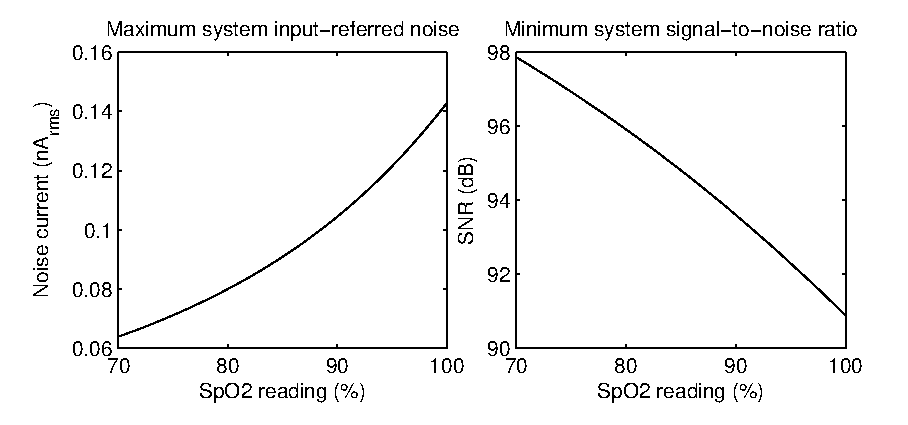
\includegraphics[scale=1]{kuvat/noise_requirement_vs_spo2_fft}
    \caption{Acceptable system noise level as a function of \spo reading when using an algorithm that's based on a 64-point FFT and values from table \ref{tbl:specification_constants}.}
    \label{fig:noise_requirement_vs_spo2_fft}
  \end{center}
\end{figure}

\subsection{Timing and Channel Noise Correlation}

The scenario portrayed in the previous section assumes that the measurement noises present in the different channels drive R towards the same direction instead of countering each other. It's to be noted, though, that as a single receiver chain is used to measure all four channels (red, infrared, red ambient, infrared ambient) it's probable that most of the noise is common for them, and equation (\ref{eq:DeltaR}) shows that the more correlated the channel noises are the smaller the effect on R is in typical operating conditions.

A feature that helps to reduce uncorrelated noise is oversampling. The sampling frequency can be anywhere between 100 Hz and 1000 Hz, the output filtered and downsampled to the target sample rate, usually 40-100 Hz. When N samples of a DC signal are summed together the result is N times larger but the uncorrelated noise only increases by a factor of $\sqrt{N}$, causing the total signal-to-noise ratio to also increase by $\sqrt{N}$. This is why all noise in this thesis is examined in the target bandwidth of 0.5-20 Hz without taking the actual Nyquist frequency of the raw signal into account.

\subsection{Noise Sources}

If the system is designed optimally there's no single big noise source in the system that could be directly pinpointed but instead every subsystem in the signal chain adds its own contribution into the total system noise. Most of this is plain thermal noise found in all conductors but each subsystem also exhibits some special behavior that should be taken into account in the design and verification.

\subsubsection{LED Current Regulator}

The transmitter, or LED drive, regulates the pulsed current directed into the LEDs. Typically the control reference is given by an 8-bit DAC which transfers a digital value into a reference voltage that guides the current regulator. Now, the important feature of the DAC isn't the resolution it provides (8 bits is well enough) but the repeatability of the conversion result -- it is imperative that two current pulses of same reference setting are regulated with the same reference voltage since all variation between the pulses will directly translate into variation between measured samples. For this same reason the noise of the band gap providing a reference for the DAC has to be as small as possible.

All in all, with current technology it's reasonably easy to build a cost-effective LED drive that has a signal-to-noise ratio of 115 dB, which is the design specification of the transmitter in the new design. The 115 dB specification ensures that the transmitter noise is well below receiver noise and can often be treated as non-existent.

\subsubsection{Photodetector}

Noise in a photodiode is primarily due to shot noise -- the random generation of carriers within the P-N junction also yields random current. Negatively biasing the photodiode increases the response speed and sensitivity of the detector but also increases noise \cite{OSIOptoelectronics}, due to which GE uses non-biased detectors. In general as the detector is the source of signal in the receiver chain its noise behavior defines the minimum detectable power of the whole system.

\subsubsection{Trans-Impedance Amplifier}

A trans-impedance amplifier transforms a current signal into a voltage one. It is usually implemented with an operational amplifier with the voltage over a resistor the current flows through as the input. Even though the system's input is differential, due to the length of the sensor cable and noisy environment it is still possible that large induced voltages are present as a common-mode disturbance. Due to this it is important that the op-amp selected has a good common-mode rejection ratio (CMRR) in addition to low overall noise. For the higher-end amplifiers of National Semiconductor typical CMRR values are in the range of 130 dB and input noise ca.\ 3.3 $nV/\sqrt{Hz}$ \cite{nationalLMP7731}.

As \cite{Schwartz1990} states, the power of a noise signal isn't changed by sampling; therefore when calculating the SNR of the op-amp, the full bandwidth, which in turn is defined by sampling rate, must be taken into account. For a sampling rate of 625 Hz the SNR of the part above for a signal of 0.5 V would be in the range of 135 dB which is well above the specification of the whole system. In any case, due to the feedback circuit the output noise of the operational amplifier usually has a linear relationship to its gain, namely the feedback resistor.

\subsubsection{Sample-and-Hold}

A sample-and-hold block is most commonly implemented as a switched capacitor circuit working in two phases: during sampling phase the input is switched in to charge the sampling capacitor and during hold phase the voltage of the capacitor is buffered to output. Therefore the effective noise of the circuit can be broken into sampling noise and hold-time continuous noise as well. \cite{Gai2008}

As the hold-time noise is usually of little significance, only sampling noise is handled here. The primary source for it is that the sampling circuit's thermal noise introduces a random component in the sampled signal: the sampling capacitor will hold the voltage that the input had when the switch was opened. As the high-pass filtering properties of the capacitor are related to its capacitance, the sampling noise can be formulated as \cite{Gai2008}
\begin{equation}
  V_{nRMS} = \sqrt{\frac{k_BT}{C}} .
\end{equation}

This leads to the fact that careful thought must be put into selecting the capacitor: a small capacitor offers a fast response allowing for short sampling times but introduces more noise than a bigger one.

\subsubsection{A/D Conversion}

Most A/D converters tend to be sigma-delta types. They operate at a much higher frequency than the actual sampling and conversion frequency and use a feedback loop comparing the latest result to the input signal level \cite{Aziz1996}. For accurate operation the converter needs a stable reference voltage, an accurate clock and a noise-free input. As all analog-to-digital conversions show quantization noise a completely noise-free conversion is impossible; the relative quantization noise in signals close to zero could be diminished by utilizing a logarithmic conversion scale but due to practical reasons concerning signal post-processing it is rarely used.

\subsubsection{Ambient Light}

Although the measurement site can be shielded with an opaque shell covering the sensor, it's still highly probable that some ambient light still finds its way to the photodetector. This can be a problem especially in operating room conditions where high intensity illumination is required. The noise caused by ambient light is typically double line frequency (100 or 120 Hz) noise with a DC component, thus disturbing both the AC and the DC measurement. This is why the ambient level is sampled as well and subtracted from the red and infrared measurements. In addition to removing the ambient effect the subtraction also removes other correlated low frequency noise from the signal.